\section{Software}\label{sec:software}
Wichtig für dieses Kapitel ist, dass der beschriebene Zustand der Software dem Soll-Zustand entspricht. Die Abweichungen sind im Kapitel Validierung genauer beschrieben.

Es wird ein NRF52832 verwendet von Nordic Semiconductor. Dadurch liegt die Verwendung des Software Development Kit \cite{nordic_sdk} nahe. Dies ist eine Sammlung von Beispielen, Librarys und vorcompilierten Codes. Nachfolgend wird das Software Development Kit nur noch SDK genannt. Es wurde nRF5 SDK v12.3.0 verwendet. Wichtig ist die SDK für ihren integrierten Bluetooth-Stack, der verwendet wird. Dieser ist im sogenannten Softdevice enthalten. Um ihn nutzen zu können, verwenden wir den S132. Dieser und die nötige Initialisierungen des Bluetooth-Stacks waren in dem Beispielprojekt Uartc in der Central-Rolle vorhanden. Dadurch wurde das ganze Projekt auf diesem Beispiel aufgebaut. Der Softdevice und die SDK legen einige abstraktions Layer auf die Hardware. Diese sind in Abbildung \ref{fig:Software_Layers} visualisiert. Die wichtigsten Module des SDK werden im Kapitel \ref{sec:nordicsdk} erklärt, falls weitere Informationen gewünscht sind wird auf die offizielle Dokumentation verwiesen \cite{nordic_info}.

\begin{figure}[htbp!!!!]
	\centering
	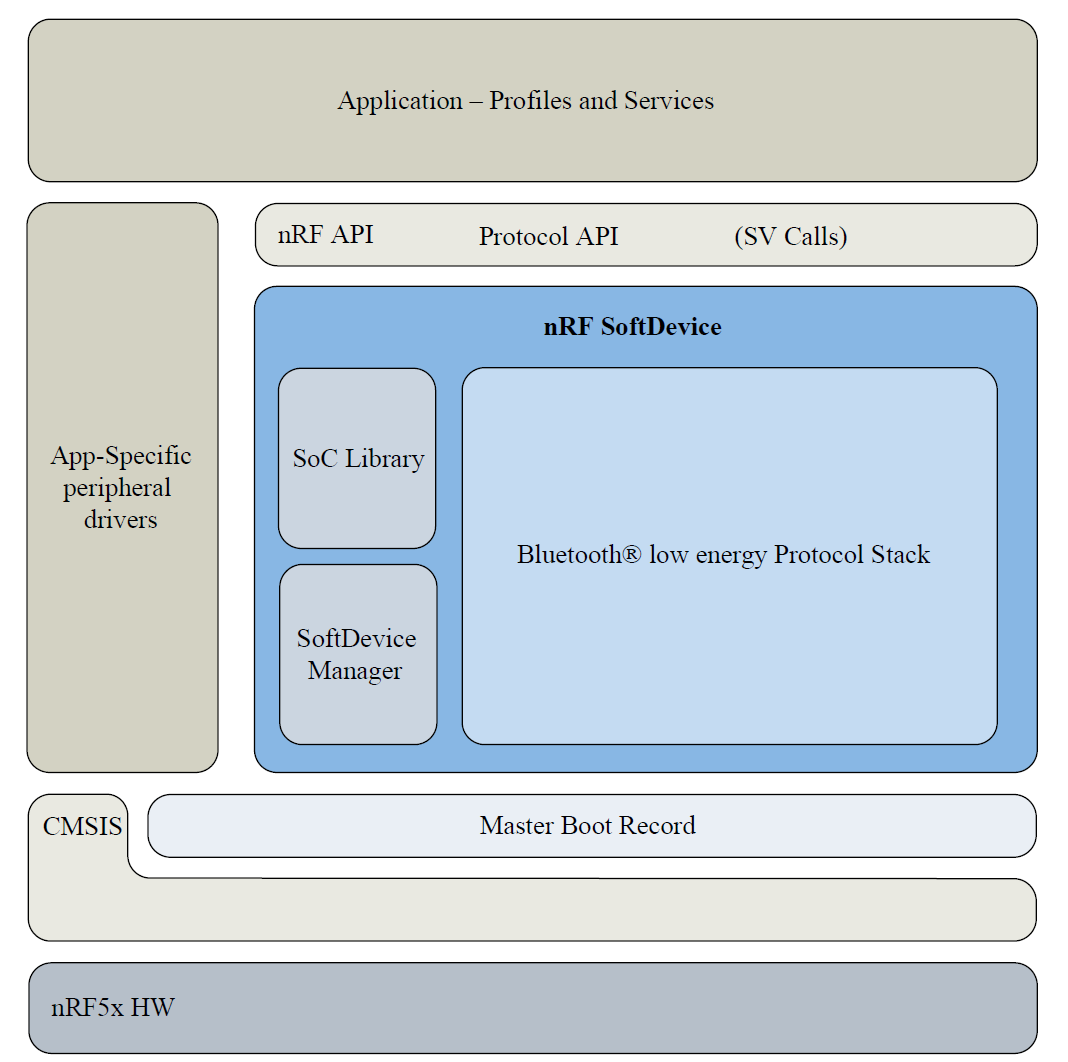
\includegraphics[width=0.7\textwidth]{Data/Software_Layers.PNG}
	\caption[Software:Layers]{Aufbau der Software auf der Hardware}
	\label{fig:Software_Layers}
\end{figure} 

Der eigentliche Programmaufbau ist eine Statmachine. Diese ist in einem separaten Kapitel erläutert. Das Programm ist so aufgebaut, dass alle Events möglichst kurz gehalten wurden. Jedoch hat dies relativ viele Flags zur folge. Anschliessend werden die die Events entsprechend ihrer Priorität verarbeitet. Die Prioritäten ergeben sich aus der Else IF im Wait State, genauers im Kapitel \ref{sec:stateMachine}. Dadurch entsteht ein pollendes Programm mit Prioritäten, was in Abbildung \ref{fig:Software_approach} dargestellt ist.

\begin{figure}[htbp!!!!]
	\centering
	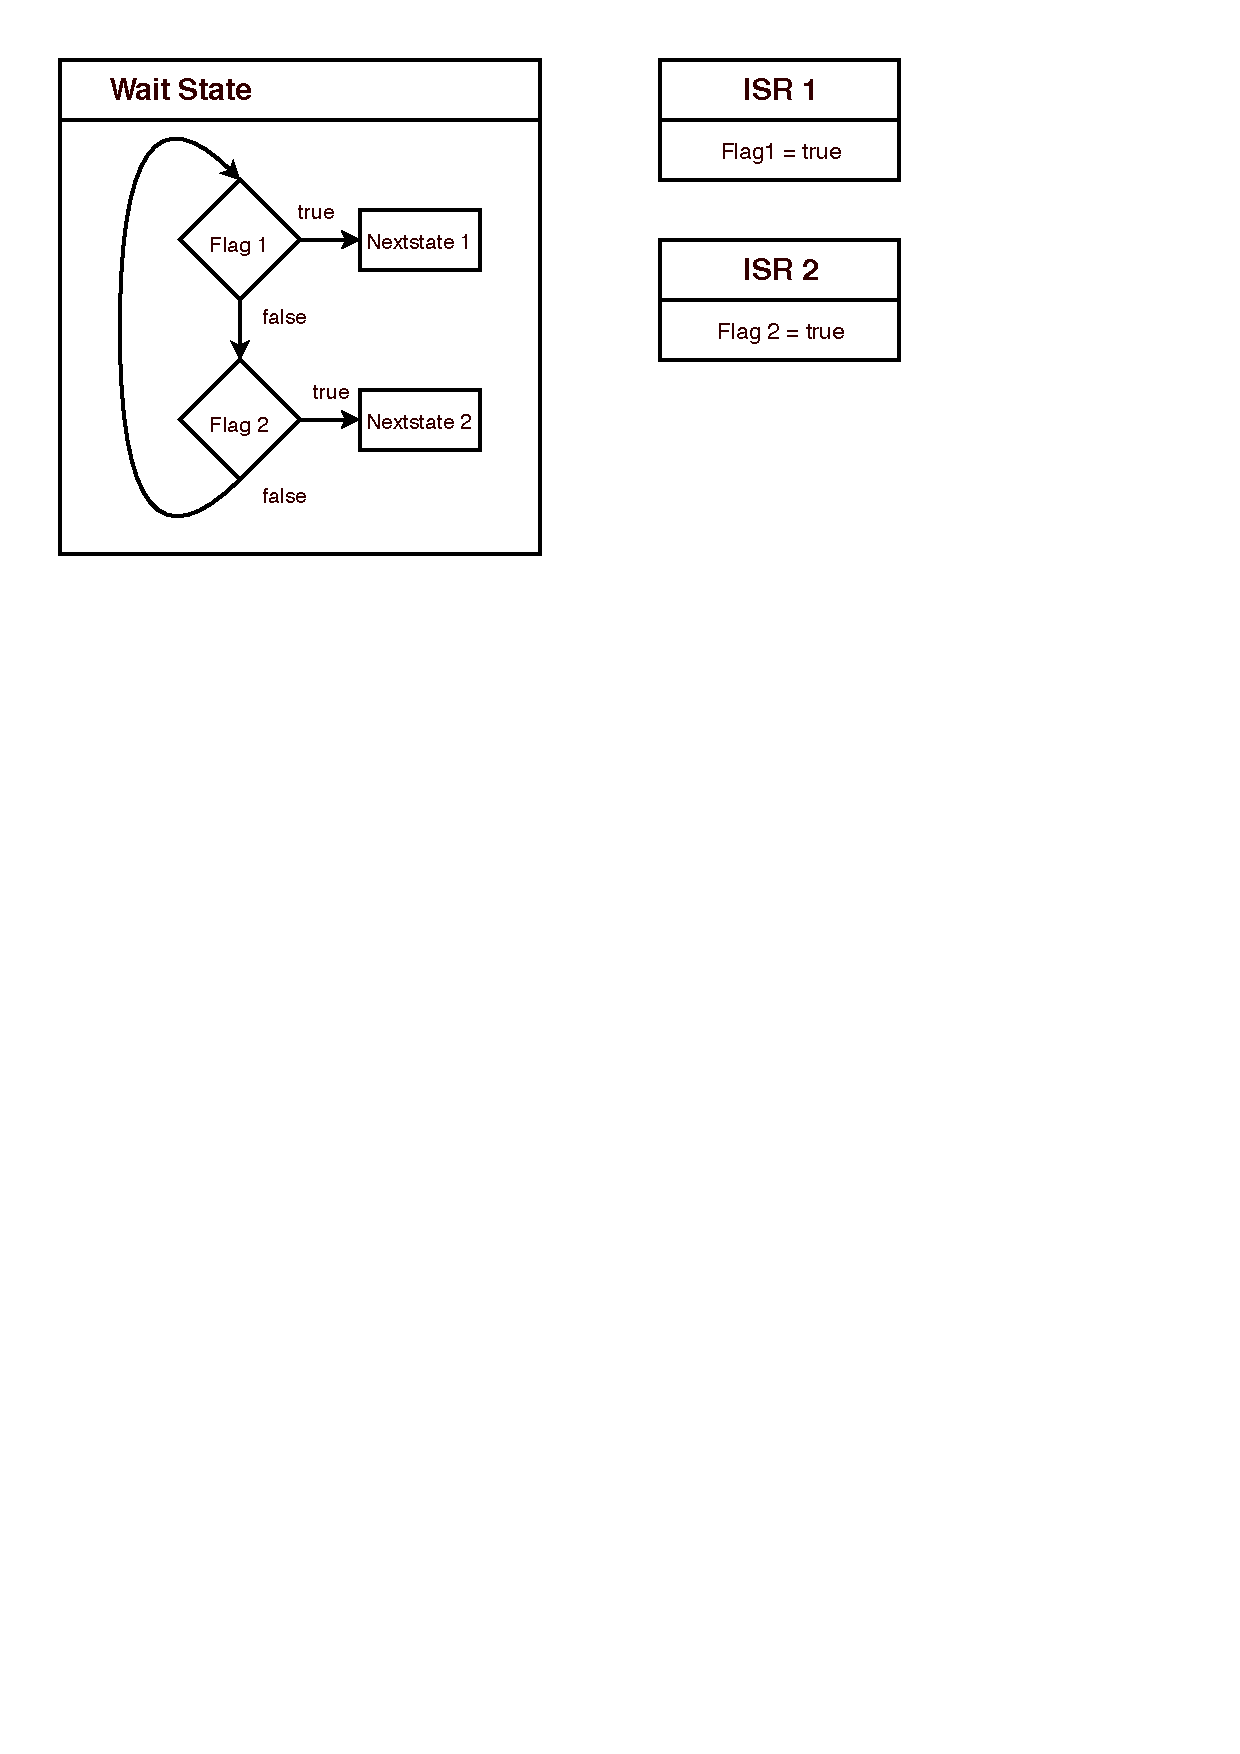
\includegraphics[width=0.7\textwidth]{Data/Software_Pollend.pdf}
	\caption[Software:Pollend]{Konzept der pollenden Software}
	\label{fig:Software_approach}
\end{figure}

Das Programm wurde in verschiedene Module unterteilt, um die Leserlichkeit zu verbessern. Die Unterteilung wurde entsprechend der Funktion gemacht. Im Hauptmodul (Main) ist nur die Statmachine und die Interrupthandler vorhanden. Folglich wurde ein Modul für die BLE-Funktionalitäten geschrieben und eines für die SD-Karte. Ein weiters existiert für die Batterie-Funktionalitäten. Dieses ist jedoch nicht implementiert und enthält nur Dummy-Funktionen.






